\section{Audit of 92 Agent-Engineered Clinical Features}
\label{sec:agentic_fe}

Autonomous domain agents reviewed cardiothoracic POAF physiology~\cite{dobrev2019postoperative,mariscalco2014poaf,burgos2021comaf} and the STS v2.81 codebook~\cite{sts2014v281}, authoring and unit-testing \textbf{92 strictly pre-incision features} across three tracks (complete taxonomy and auxiliary AUCs in Appendix~D):
\begin{enumerate}
  \item \textbf{Track~1 (58 features):} Pre-incision proxies of bedside scores (Mariscalco POAF~\cite{mariscalco2014poaf}, COM-AF~\cite{burgos2021comaf}, $\mathrm{CHA_2DS_2\text{-}VASc}$~\cite{lip2010cha2ds2vasc}, HATCH~\cite{devos2010hatch}, Mathew~\cite{mathew2004multicenter}) plus continuous organ-reserve biomarkers (CKD-EPI 2021 eGFR~\cite{inker2021ckdepi}, ALBI hepatic grade~\cite{johnson2015albi}, anemia severity, biatrial remodeling proxies, acute $\beta$-blocker withdrawal). Note that STS-reconstructed scores are domain proxies where registry definitions substitute or omit original inputs.
  \item \textbf{Track~2A (24 features):} Nonlinear physiological interactions (\cli{diabetes\_age\_decoupled}, age--sex--BSA--race atrial substrate gradients, HFpEF diastolic substrate, prior revascularization burden, cardiorenal--anemia triad).
  \item \textbf{Track~2B (10 features):} Strictly nested hospital-grouped OOF risk logits for the eight clean auxiliary STS complications (e.g., renal failure AUC 0.8365, mortality 0.8048, prolonged ventilation 0.7653) plus two systemic-cascade composites.
\end{enumerate}

\begin{figure*}[t]
  \centering
  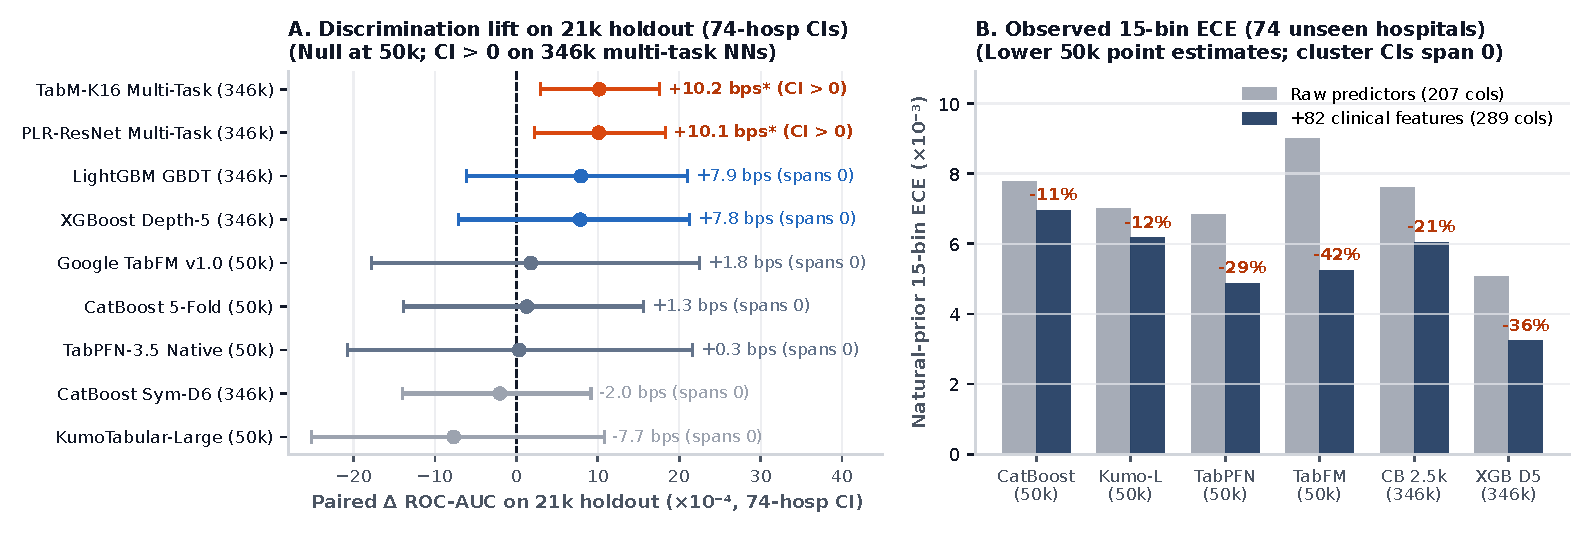
\includegraphics[width=\textwidth]{figures/fig3_agentic_fe_lift_and_calibration.pdf}
  \caption{\ct{Cross-paradigm audit of 82 deterministic clinical features (289 vs.\ 207 raw predictors) strictly on \cli{test\_full\_21k} ($N=21{,}241$, 74 unseen hospitals).} \textbf{(A)}~Paired $\Delta$ROC-AUC with 5,000-draw 74-hospital cluster 95\% intervals shows null lift on all 50k models, but intervals strictly above zero on 346k multi-task neural networks. \textbf{(B)}~Observed natural-prior 15-bin ECE point estimates fall 11\%--42\% across all four tested 50k families (plus 346k default CatBoost and XGBoost), though 74-hospital cluster ECE intervals span zero.}
  \label{fig:agentic_fe}
\end{figure*}

\runin{Empirical verdict}
Comparing raw 207-feature matrices against the 289-feature bundle (207 raw $+$ 82 deterministic Track~1/2A features) strictly on the primary natural-prior holdout (\cli{test\_full\_21k}, $N=21{,}241$, 74 unseen centers) across both cohort scales yields three clear findings (Figure~\ref{fig:agentic_fe}):
\begin{itemize}
  \item \textbf{Null discrimination lift on 50k trees and TFMs:} Under dual-GBDT CV screening, only 1 of 92 features passed promotion (\cli{diabetes\_age\_decoupled}; 0/58 Track~1, 0/10 Track~2B). Strictly on \cli{test\_full\_21k} at $N=50{,}000$, adding all 82 clinical features left ROC-AUC flat on CatBoost ($+0.00013$ $[-0.00138, +0.00156]$), TabPFN-3.5 Native ($+0.00003$ $[-0.00207, +0.00216]$), KumoTabular-Large ($-0.00077$ $[-0.00251, +0.00108]$), and TabFM ($+0.00018$ $[-0.00178, +0.00225]$), and similarly flat on 346k CatBoost ($-0.00039$ on 2.5k-tree / $-0.00020$ on 3.5k-tree configs). Tellingly, CatBoost still ranked engineered composites \#1--\#5 in feature importance, showing that large tree ensembles already approximate additive bedside scores from raw covariates.
  \item \textbf{Lower observed 15-bin ECE across tested 50k families (with wide cluster uncertainty):} Despite flat AUC, adding the 82 clinical features lowered observed natural-prior 15-bin ECE~\cite{guo2017calibration,vancalster2019calibration} point estimates across all four tested 50k families by \textbf{11\%--42\%}---CatBoost 50k ($0.00778 \to 0.00695$, $-11\%$), KumoTabular ($0.00702 \to 0.00617$, $-12\%$), TabPFN-3.5 Native ($0.00683 \to 0.00488$, $-29\%$), and TabFM v1.0.0 ($0.00901 \to 0.00524$, $-42\%$)---as well as 346k default 2.5k-tree CatBoost ($0.00760 \to 0.00604$, $-21\%$) and XGBoost ($0.00507 \to 0.00323$, $-36\%$). Crucially, 5,000-draw 74-hospital cluster intervals on these 50k ECE shifts all span zero (and Brier/LogLoss shifts were mixed across families), while at 346k deeper 3.5k-tree CatBoost ($0.00592 \to 0.00633$), LightGBM ($0.00411 \to 0.00456$), and PLR-ResNet ($0.01135 \to 0.01260$) showed slightly higher ECE despite improved LogLoss and Brier.
  \item \textbf{Hospital-cluster-confirmed neural lift at 346k:} At full registry scale ($N=346{,}454$), explicit clinical features lifted multi-task deep tabular networks~\cite{caruana1997multitask,gorishniy2022embeddings,gorishniy2025tabm} with 74-hospital 95\% intervals strictly above zero: TabM-K16 MultiTask ($+0.00102$ $[+0.00029, +0.00176]$, 99.6\% positive draws) and PLR-ResNet MultiTask ($+0.00101$ $[+0.00022, +0.00183]$, 99.4\%), alongside non-significant positive trends on leaf-wise LightGBM ($+0.00079$) and XGBoost ($+0.00078$).
\end{itemize}
In summary, agentic clinical feature engineering does not lift 50k binary-label discrimination on this 207-variable registry, yields lower observed 15-bin ECE point estimates at 50k (without excluding zero under hospital clustering), and provides hospital-cluster-confirmed representation gains for full-registry multi-task neural networks. Because engineered inputs leave 50k binary-label discrimination flat across trees and foundation models alike, we next test whether the limiting bottleneck lies in binary $\{0,1\}$ supervision itself (\S\ref{sec:benchmarks}).
